%% Customizações do abnTeX2 (http://www.abntex.net.br) para o Instituto de Matemática,
%% Estatística e Computação Científica da Universidade Estadual de Campinas (IMECC-UNICAMP)
%%
%% 2022 - Esta versão está compatível com a Instrução Normativa CCPG nº 002/2021
%%
%% This work may be distributed and/or modified under the conditions of the LaTeX Project
%% Public License, either version 1.3 of this license or (at your option) any later version.
%% The latest version of this license is in http://www.latex-project.org/lppl.txt and version
%% 1.3 or later is part of all distributions of LaTeX version 2005/12/01 or later.
%%
%% This work has the LPPL maintenance status `maintained'.
%% 
%% The Current Maintainer of this work is Fábio Rodrigues Silva, gfabinhomat@gmail.com
%%
%% Further information about abnTeX2 are available on http://www.abntex.net.br
%%
\documentclass[
	oldfontcommands,
	% -- opções de customização --
	sumario=tradicional,
	%sumario=abnt-6027-2012,
	% -- opções da classe memoir --
	12pt,			% tamanho da fonte
	openright,		% capítulos começam em pág ímpar (insere página vazia caso preciso)
	oneside,		% impressão em anverso (norma CCPG).
	a4paper,		% tamanho do papel. 
	% -- opções da classe abntex2 --
	%chapter=TITLE,		% títulos de capítulos convertidos em letras maiúsculas
	%section=TITLE,		% títulos de seções convertidos em letras maiúsculas
	%subsection=TITLE,	% títulos de subseções convertidos em letras maiúsculas
	%subsubsection=TITLE,	% títulos de subsubseções convertidos em letras maiúsculas
	% -- opções do pacote babel --
	english,		% idioma adicional para hifenização
	english			% o último idioma é o principal do documento
	]{imecc-unicamp}
% ----------------------------------------------------------
% PACOTES ESSENCIAIS
% pacotes básicos (essenciais ao modelo). NÃO RETIRAR NENHUM
	\usepackage{lmodern}            % Usa a fonte Latin Modern
	\usepackage[T1]{fontenc}        % Seleção de códigos de fonte.
	\usepackage[utf8]{inputenc}     % Codificação do documento (conversão automática dos acentos)
	\usepackage{lastpage}           % Usado pela Ficha catalográfica
	\usepackage{indentfirst}        % Indenta o primeiro parágrafo de cada seção.
	\usepackage{color,xcolor}       % Controle das cores
	\usepackage{graphicx}           % Inclusão de gráficos
	\usepackage{microtype}          % para melhorias de justificação
	\usepackage{hyperref}           % Amplo suporte para hipertexto em LaTeX
	\usepackage[brazilian]{backref} % Paginas com as citações na bibl
	\usepackage[alf,
			abnt-repeated-author-omit=yes,
			abnt-etal-list=0]{abntex2cite} % Citações padrão ABNT
	
% pacotes sugeridos
	\usepackage{lipsum}   % Textos de teste
	\usepackage{enumitem} % Auxiliar dos ambientes itemize, enumerate e description
	\usepackage{amsfonts} % Fontes AMS
	\usepackage{amsmath}  % Facilidades matemáticas
	\usepackage{tikz}     % Para desenhos e diagramas
	\usepackage{bm}       % Para a função \boldsymbol{} que escreve em negrito no modo matemático
	\usepackage{icomma}   % Remove os espaços após a vírgula no modo matemático (a menos que especificado)

	% \usepackage{verbatim}
	% \usepackage{float}
	% \usepackage{amsbsy}   % Para símbolos matemáticos em negrito
	% \usepackage{amscd}    % Para diagramas
	% \usepackage{amssymb}  % Para os símbolos mais antigos
	% \usepackage{amstext}  % Para fragmentos tipo texto em modo matemático
	% \usepackage{amsthm}   % Para teoremas
	% \usepackage{cleveref} % Referência cruzada inteligente
	% \usepackage{dsfont}   % Para o estilo de conjuntos de números $\mathds{R}$
	% \usepackage{ifthen}   % Comandos de condição em LaTeX
	% \usepackage{listings} % Para inserir códigos de outras linguagens de programação
	% \usepackage{lscape}   % Para imprimir alguma página no formato paisagem
	% \usepackage{mathabx}  % Conjunto de símbolos matemáticos
	% \usepackage{mathrsfs} % Suporte para fontes RSFS
	% \usepackage{pdfpages} % Para inserir páginas PDF no texto
	% \usepackage{subfig}   % Para figuras lado-a-lado
	% \usepackage[english,onelanguage]{algorithm2e} % Para inserir algoritmos (longend,vlined)

% ----------------------------------------------------------
% ----------------------------------------------------------
% INFORMAÇÕES E DADOS PARA CAPA E FOLHA DE ROSTO
% Informações gerais do trabalho EM LÍNGUA PORTUGUESA
	\titulo{Título da sua Dissertação de Mestrado ou Tese de Doutorado}
	\tipotrabalho{Dissertação} % ou Tese
	\curso{Estatística} % ou Matemática ou Matemática Aplicada ou Matemática Aplicada e Computacional
	% \curso{}  % Se for aluno do PROFMAT
	
% Suas informações NA LÍNGUA DO TRABALHO
	% Aluno do sexo MASCULINO:
	% \autor{Nome Completo do Aluno}
	% \titulacao{Mestre} % ou Doutor
	% Aluna do sexo FEMININO
	\autor[autora]{Nome Completo da Aluna}
	\titulacao{Mestra} % ou Doutora
	% orientador/coorientador do sexo MASCULINO
	% \orientador{Nome Completo do Orientador}
	% \coorientador{Nome Completo do Coorientador}
	% orientador/coorientador do sexo FEMININO (exceto se o trabalho for em inglês)
	\orientador[Orientadora]{Nome Completo da Orientadora}
	\coorientador[Coorientadora]{Nome Completo da Coorientadora}
	
% Data
	\data{Ano da banca}

% ----------------------------------------------------------
% ----------------------------------------------------------
% CONFIGURAÇÕES GERAIS
% As configurações gerais são colocadas aqui, como novos comandos para o corpo do texto,
% informações de bookmark para o PDF, tamanho de parágrafos, entre outros.

% Formatação em geral
	% Formataçao da página
	\setlength{\parindent}{2.0cm} % O tamanho do parágrafo
	\setlength{\parskip}{0.2cm}  % tente também \onelineskip. Controle do espaçamento entre um parágrafo e outro
	
	% Formatação dos nomes nas seções
	% \chapterstyle{default} % Para que apareça o nome 'Capítulo X' antes do título de cada capítulo
	
	% Formatação do modo matemático
	\everymath{\displaystyle} % Com isso você não precisa se preocupar com a localização dos limitantes dos somatórios etc ($$\sum_{i = 1}^{n}$$)
	
	% cores
	\definecolor{blue}{RGB}{41,5,195}
	\definecolor{verde}{rgb}{0,0.5,0}
	
	% cores adicionais
	% Na minha dissertação eu optei por usar essas duas paletas de cores em várias situações sinta-se livre para modificar ou usar.
	% Pelo que me lembro, usei como base o site colorbrewer2.org
	\definecolor{pal1.1}{HTML}{8DA0CB}
	\definecolor{pal1.2}{HTML}{66C2A5}
	\definecolor{pal1.3}{HTML}{FC8D62}
	
	\definecolor{pal2.1}{HTML}{e41a1c}
	\definecolor{pal2.2}{HTML}{ff7f00}
	\definecolor{pal2.3}{HTML}{984ea3}
	\definecolor{pal2.4}{HTML}{377eb8}
	\definecolor{pal2.5}{HTML}{4daf4a}

% Novos comandos e ambientes
	% para facilitar com os pacotes
	\newcommand{\citep}{\citeonline} % Na minha dissertação usei o padrção de referências Nome Do Fulano (1999). Com esse ajuste você pode usar só o \citep{apelido_do_artigo}
	
	% Tikz - Usei muito esse exemplo de boxplot aqui nas legendas. Você pode apagar, modificar, etc.
	\newcommand{\boxplotLegenda}[1]{\tikz[scale=0.2, baseline = {(0ex, -0.5ex)}]{
		\filldraw[#1, draw = black] (0, -.5) rectangle +(1, 1.3);
		\draw[very thick] (0, -.1) -- +(1, 0);
		\draw (.5,-.5) -- +(0, -.2);
		\draw (.25,-.7) -- +(.5, 0);
		\draw (.5,.8) -- +(0, .4);
		\draw (.25,1.2) -- +(.5, 0);}}
	
	% Ambientes personalizados
	% \theoremstyle{plain}
	\newtheorem{theorem}{Teorema}%[chapter]
	\newtheorem{corollary}{Corolário}%[chapter]
	\providecommand*{\corollaryautorefname}{Corolário}
	\newtheorem{conjecture}{Conjectura}%[chapter]
	\providecommand*{\definitionautorefname}{Definição}
	\newtheorem{example}{Exemplo}%[chapter]
	\providecommand*{\exampleautorefname}{Exemplo}
	
	% Operadores abreviados
	\DeclareMathOperator{\argmin}{\mathrm{arg}\min}
	\DeclareMathOperator{\argmax}{\mathrm{arg}\max}
	\DeclareMathOperator{\sgn}{\mathrm{sgn}}
	\renewcommand{\sin}{\mathrm{sen}}
	\renewcommand{\tan}{\mathrm{tg}}
	\renewcommand{\csc}{\mathrm{cossec}}
	\renewcommand{\cot}{\mathrm{cotg}}

% Configurações de pacores
	% backref (recomendo não mexer)
		% Usado sem a opção hyperpageref de backref
		\renewcommand{\backrefpagesname}{Citado na(s) página(s):~}
		% Texto padrão antes do número das páginas
		\renewcommand{\backref}{}
		% Define os textos da citação
		\renewcommand*{\backrefalt}[4]{
			\ifcase #1 %
				Nenhuma citação no texto.%
			\or
				Citado na página #2.%
			\else
				Citado #1 vezes nas páginas #2.%
			\fi}

	% chngcntr
		\counterwithin{figure}{chapter} % Figuras enumeradas segundo o capítulo
		\counterwithin{table}{chapter} % Tabelas enumeradas segundo o capítulo

	% listings
		%\lstset{
		%	language=C++,
		%	basicstyle=\ttfamily, 
		%	keywordstyle=\color{blue}, 
		%	stringstyle=\color{verde}, 
		%	commentstyle=\color{red}, 
		%	extendedchars=true, 
		%	showspaces=false, 
		%	showstringspaces=false,
		%	numbers=left,
		%	numberstyle=\tiny,
		%	breaklines=true, 
		%	backgroundcolor=\color{green!10},
		%	breakautoindent=true,
		%	fontadjust=false
		%}
		
	% hyperref (recomendo não mexer)
		\makeatletter
		\hypersetup{
			%pagebackref=true,
			pdftitle={\@title},
			pdfauthor={\@author},
			pdfsubject={%
				\imprimirtipotrabalho\ apresentada ao Instituto de Matemática, Estatística %
				e Computação Científica da Universidade Estadual de Campinas como parte dos %
				requisitos exigidos para a obtenção do título de \imprimirtitulacao\ em %
				\imprimircurso.
			},
			pdfcreator={LaTeX with unicamp-abnTeX2},
			pdfkeywords={abnt}{latex}{abntex}{abntex2}{trabalho acadêmico},
			colorlinks=true,   % false: boxed links; true: colored links
			linkcolor=blue,    % color of internal links
			citecolor=blue,    % color of links to bibliography
			filecolor=magenta, % color of file links
			urlcolor=blue,     % color of internet links
			bookmarksdepth=4
		}
		\makeatother
% Gerenciamento de arquivos
	% Gerenciamento de pastas
	\graphicspath{{figuras/}} % Faz com que você não precise se referir à pasta figuras quando chamar no \includegraphics.

% ?
	\newsubfloat{figure} % Allow subfloats in figure environment
	\providecommand*{\subfigureautorefname}{Subfigura}

% ----------------------------------------------------------
% -----------------------------------------------------------------------------------------------
% %%%%%%%%%%%%%%%%%%%%%%%%%%%%%%%%%%%%% INÍCIO DO DOCUMENTO %%%%%%%%%%%%%%%%%%%%%%%%%%%%%%%%%%%%%
% -----------------------------------------------------------------------------------------------
\begin{document}
% Seleciona o idioma do documento (conforme pacotes do babel)
% \selectlanguage{brazil}
\selectlanguage{english}
% Retira espaço extra obsoleto entre as frases.
\frenchspacing
% ---------------------------------------------------------------------------------
% %%%%%%%%%%%%%%%%%%%%%%% INÍCIO DOS ELEMENTOS PRÉ-TEXTUAIS %%%%%%%%%%%%%%%%%%%%%%%
% ---------------------------------------------------------------------------------
\pretextual
% ----------------------------------------------------------
% PRIMEIRA FOLHA (OBRIGATÓRIO)
\imprimirprimeirafolha
% ----------------------------------------------------------
% ----------------------------------------------------------
% FOLHA DE ROSTO (OBRIGATÓRIO)
% ---
% Após realizar as correções finais de seu trabalho acadêmico, escaneie a folha de rosto
% devidamente assinada pelo orientador e salve no formato PDF com o nome 'folha-de-rosto.pdf'
% no diretório do seu projeto. Daí substitua a linha do comando '\imprimirfolhaderosto'
% pelas 3 linhas de comando abaixo:
% ---
% \begin{folhaderosto}
%     \includepdf{folha-de-rosto.pdf}
% \end{folhaderosto}
% ---
\imprimirfolhaderosto

% ----------------------------------------------------------
% ----------------------------------------------------------
% FICHA CATALOGRÁFICA (OBRIGATÓRIO)
% ---
% A biblioteca da UNICAMP lhe fornecerá um PDF com a ficha catalográfica definitiva após a defesa
% do trabalho {http://hamal.bc.unicamp.br/catalogonline2/}. Quando estiver com o documento, salve-o
% como PDF no diretório do seu projeto e deixe apenas o comando '\includepdf{ficha-catalografica.pdf}'
% dentro do ambiente abaixo
% ---
\begin{fichacatalografica}
    \begin{center}
	{\ABNTEXchapterfont\large A ficha catalográfica deverá ser solicitada online via \url{http://www.sbu.unicamp.br/sbu/elaboracao-de-ficha-catalografica/}}
    \end{center}
%     \includepdf{ficha-catalografica.pdf}
\end{fichacatalografica}
% ----------------------------------------------------------
% ----------------------------------------------------------
% FOLHA DE APROVAÇÃO (OBRIGATÓRIO)
% ---
% A folha de aprovação será fornecida pela secretaria de pós-graduação. Após recebê-la, escaneie a folha
% salvando em PDF no diretório do seu projeto com o nome 'folhadeaprovacao.pdf' e deixe apenas o comando
% '\includepdf{folhadeaprovacao.pdf}' dentro do ambiente abaixo
% ---
\begin{folhadeaprovacao}
    \centering{\ABNTEXchapterfont\large A folha de aprovação será fornecida pela Secretaria de Pós-Graduação}
%     \includepdf{folhadeaprovacao.pdf}
\end{folhadeaprovacao}
% ----------------------------------------------------------
% ----------------------------------------------------------
% DEDICATÓRIA (OPCIONAL)
\begin{dedicatoria}
   \vspace*{\fill}
   \centering
   \noindent
   \textit{
      Este trabalho é dedicado às crianças adultas que,\\
      quando pequenas, sonharam em se tornar cientistas.
   }
   \vspace*{\fill}
\end{dedicatoria}
% ----------------------------------------------------------
% ----------------------------------------------------------
% AGRADECIMENTOS (OPCIONAL)
\begin{agradecimentos}
Inserir aqui os agradecimentos. ATENÇÃO ALUNO BOLSISTA: você precisa mencionar agradecimento ao órgão de fomento de sua bolsa, incluindo explicitamente o código do processo. Caso seja bolsista CAPES, especial atenção ao Art. 3º da Portaria CAPES 206/2018, que prevê texto padrão de agradecimento.
\end{agradecimentos}
% ----------------------------------------------------------
% ----------------------------------------------------------
% EPÍGRAFE (OPCIONAL)
\begin{epigrafe}
    \vspace*{\fill}
    \begin{flushright}
	\textit{``Não vos amoldeis às estruturas deste mundo, \\
	    mas transformai-vos pela renovação da mente, \\
	    a fim de distinguir qual é a vontade de Deus: \\
	    o que é bom, o que Lhe é agradável, o que é perfeito.\\
	    (Bíblia Sagrada, Romanos 12, 2)
	}
    \end{flushright}
\end{epigrafe}
% ----------------------------------------------------------
% ----------------------------------------------------------
% RESUMOS (OBRIGATÓRIO)
% -------------------------------------------------------------
%  RESUMOS
\setlength{\absparsep}{18pt} % ajusta o espaçamento dos parágrafos do resumo
% -------------------------------------------------------------
% ATENÇÃO: o ambiente 'otherlanguage*' deve ser usado para o resumo que não está na
% língua vernácula do trabalho, com a respectiva opção linguística do pacote 'babel'.
% -------------------------------------------------------------
% resumo em PORTUGUÊS (OBRIGATÓRIO)
\begin{resumo}[Resumo]
 \begin{otherlanguage*}{brazil}
    Segundo a \citeonline[3.1-3.2]{NBR6028:2003}, o resumo deve ressaltar o objetivo,
    o método, os resultados e as conclusões do documento. A ordem e a extensão destes
    itens dependem do tipo de resumo (informativo ou indicativo) e do tratamento que
    cada item recebe no documento original. O resumo deve ser precedido da referência
    do documento, com exceção do resumo inserido no próprio documento. Neste trabalho,
    devem ser utilizadas até 500 palavras. (\ldots) As palavras-chave devem figurar
    logo abaixo do resumo, antecedidas da expressão Palavras-chave:, separadas entre
    si por ponto e finalizadas também por ponto.

    \textbf{Palavras-chave}: Latex. Abntex. Editoração de texto.
 \end{otherlanguage*}
\end{resumo}
% -------------------------------------------------------------
% -------------------------------------------------------------
% resumo em INGLÊS (OBRIGATÓRIO)
\begin{resumo}[Abstract]
 \begin{otherlanguage*}{english}
    This is the english abstract.
    
    \textbf{Keywords}: Latex. Abntex. Text editoration.
 \end{otherlanguage*}
\end{resumo}
% -------------------------------------------------------------
% ----------------------------------------------------------
% ----------------------------------------------------------
% LISTA DE ILUSTRAÇÕES (OPCIONAL)
\pdfbookmark[0]{\listfigurename}{lof}
\listoffigures*
\cleardoublepage
% ----------------------------------------------------------
% ----------------------------------------------------------
% LISTA DE TABELAS (OPCIONAL)
\pdfbookmark[0]{\listtablename}{lot}
\listoftables*
\cleardoublepage
% ----------------------------------------------------------
% ----------------------------------------------------------
% LISTA DE ABREVIATURAS E SIGLAS (OPCIONAL)
\begin{siglas}
  \item[UNICAMP] Universidade Estadual de Campinas
  \item[IMECC] Instituto de Matemática, Estatística e Computação Científica
  \item[LabCSD] Laboratório de Controle e Sistemas Dinâmicos
  \item[EPIFISMA] Laboratório de Epidemiologia e Fisiologia Matemática
  \item[LCP] Laboratório de Computação Paralela
  \item[LGC] Laboratório de Geofísica Computacional
  \item[LMDC] Laboratório de Matemática Discreta e Códigos
  \item[MiLAB] Laboratório de Tratamento Matemático de Imagens e Inteligência Computacional
  \item[LPOO] Laboratório de Pesquisa Operacional e Otimização
  \item[LEM] Laboratório de Ensino de Matemática
  \item[PAPMEM] Programa de Aperfeiçoamento para Professores de Matemática do Ensino Médio
  \item[OMU] Olimpíada de Matemática da Unicamp
  \item[CCPG] Comissão Central de Pós-Graduação
  \item[ABNT] Associação Brasileira de Normas Técnicas
  \item[abnTeX] ABsurdas Normas para TeX
\end{siglas}
% ----------------------------------------------------------
% ----------------------------------------------------------
% LISTA DE SÍMBOLOS (OPCIONAL)
\begin{simbolos}
  \item[$ \mathds{M}_{m\times n}(\mathds{R}) $] Conjunto das matrizes de ordem $m\times n$ com entradas reais
  \item[$ \mathds{R}^n_+ $] Conjunto dos vetores $x$ pertencentes a $\mathds{R}^n$ que satisfazem $x\geq0$
  \item[$ \mathds{R}^n_{++} $] Conjunto dos vetores $x$ pertencentes a $\mathds{R}^n$ que satisfazem $x>0$
  \item[$\|\cdot\|$] Norma-p vetorial
  \item[$\vvvert\cdot\vvvert_p$] Norma-p matricial
  \item[$\mathbf{I}_n$] Matriz identidade de ordem $n \times n$
  \item[$\nabla f$] Gradiente da função $f$
  \item[$\infty$] Infinito
\end{simbolos}
% ----------------------------------------------------------
% ----------------------------------------------------------
% LISTA DE ALGORITMOS (OPCIONAL)
\pdfbookmark[0]{\listalgorithmcfname}{loa}
\listofalgorithms
\cleardoublepage
% ----------------------------------------------------------
% ----------------------------------------------------------
% LISTA DE CÓDIGOS (OPCIONAL)
\pdfbookmark[0]{\lstlistlistingname}{lol}
\begin{KeepFromToc}
\lstlistoflistings
\end{KeepFromToc}
\cleardoublepage
% ----------------------------------------------------------
% ----------------------------------------------------------
% SUMÁRIO (OBRIGATÓRIO)
\pdfbookmark[0]{\contentsname}{toc}
\tableofcontents*
\cleardoublepage
% ----------------------------------------------------------
% ---------------------------------------------------------------------------------
% %%%%%%%%%%%%%%%%%%%%%%%% FIM DOS ELEMENTOS PRÉ-TEXTUAIS %%%%%%%%%%%%%%%%%%%%%%%%
% ---------------------------------------------------------------------------------
% ---------------------------------------------------------------------------------
% %%%%%%%%%%%%%%%%%%%%%%%%% INÍCIO DOS ELEMENTOS TEXTUAIS %%%%%%%%%%%%%%%%%%%%%%%%%
% ---------------------------------------------------------------------------------
\textual
% ----------------------------------------------------------
% INTRODUÇÃO
% ----------------------------------------------------------
% Exemplo de capítulo sem numeração, mas presente no Sumário
\chapter*[Introdução]{Introdução}
\addcontentsline{toc}{chapter}{Introdução}
% ----------------------------------------------------------

Este documento e seu código-fonte são exemplos de referência de uso da classe
\textsf{abntex2} e do pacote \textsf{abntex2cite}. O documento exemplifica a elaboração 
de trabalho acadêmico (teses e dissertações) produzido conforme a \textbf{Informação 
CCPG/001/2015} (que trata das \emph{Normas para impressão de teses/dissertações} da 
UNICAMP). Encorajamos o leitor a consultar a Informação CCPG/001/2015 \cite{CCPG:001:2015}
antes de iniciar as alterações neste documento e seu código-fonte.

A elaboração deste modelo teve como base uma customização do ``Modelo Canônico de
Trabalho Acadêmico com \abnTeX'' \cite{abntex2modelo} para que as normas presentes na
Informação CCPG/001/2015 fossem respeitadas. O modelo original produzido pela equipe 
\abnTeX\ cumpre as seguintes normas ABNT:
\begin{enumerate}
 \item \textbf{ABNT NBR 14724:2011}: Informação e documentação - Trabalhos 
    acadêmicos - Apresentação;
 \item \textbf{ABNT NBR 10520:2002}: Informação e documentação - Citações;
 \item \textbf{ABNT NBR 6034:2004}: Informação e documentação - Índice - Apresentação;
 \item \textbf{ABNT NBR 6028:2003}: Informação e documentação - Resumo - Apresentação;
 \item \textbf{ABNT NBR 6027:2012}: Informação e documentação - Sumário - Apresentação;
 \item \textbf{ABNT NBR 6024:2012}: Informação e documentação - Numeração progressiva 
    das seções de um documento - Apresentação
 \item \textbf{ABNT NBR 6023:2002}: Informação e documentação - Referência - Elaboração.
\end{enumerate}

Este documento deve ser utilizado como complemento dos manuais do \abnTeX\ 
\cite{abntex2classe,abntex2cite,abntex2cite-alf} e da classe \textsf{memoir} \cite{memoir}.

A leitura do teor desde documento (tanto o PDF quando os arquivos que compõem seu código-fonte),
bem como do arquivo \textsf{LEIAME.txt} é altamente recomendada para melhor entendimento da 
dinâmica de funcionamento da classe \textsf{abntex2} e do pacote \textsf{abntex2cite}. Seus
principais comandos e usos estão exemplificados no decorrer do texto, bem como outras informações
relevantes para a escrita de seu trabalho acadêmico.
% ----------------------------------------------------------
% DESENVOLVIMENTO
% \part{Preparação da pesquisa}
% \include{capitulo1}
% \include{capitulo2}
% \part{Referenciais teóricos}
% \include{capitulo3}
% \include{capitulo4}
% \include{capitulo5}
% \part{Resultados}
% \include{capitulo6}
% \include{capitulo7}
% --------------------
% INÍCIO DOS EXEMPLOS
% --------------------
% No âmbito do Modelo Canônico, os comandos a seguir apresentam um sucinto resumo de como
% esta classe pode ser usada. Oriente a construção do seu trabalho com base nestes comandos.
% ---
\part{Preparação da pesquisa}

% ----------------------------------------------------------
% Este capítulo, utilizado por diferentes exemplos do abnTeX2, ilustra o uso de
% comandos do abnTeX2 e de LaTeX.
% ----------------------------------------------------------
%\chapter[Title displayed in ToC][Title displayed in header]{Resultados de comandos}
\chapter{Resultados de comandos}
\label{cap_exemplos}

\chapterprecis{Isto é uma sinopse de capítulo. A ABNT não traz nenhuma
normatização a respeito desse tipo de resumo, que é mais comum em romances 
e livros técnicos.}\index{sinopse de capítulo}

% ---
\section{Codificação dos arquivos: UTF8}
% ---

A codificação de todos os arquivos do \abnTeX\ é \texttt{UTF8}. É necessário que
você utilize a mesma codificação nos documentos que escrever, inclusive nos
arquivos de base bibliográficas |.bib|.

% ---
\section{Citações diretas}
\label{sec-citacao}
% ---

\index{citações!diretas}Utilize o ambiente \texttt{citacao} para incluir
citações diretas com mais de três linhas:

\begin{citacao}
As citações diretas, no texto, com mais de três linhas, devem ser
destacadas com recuo de 4 cm da margem esquerda, com letra menor que a do texto
utilizado e sem as aspas. No caso de documentos datilografados, deve-se
observar apenas o recuo \cite[5.3]{NBR10520:2002}.
\end{citacao}

Use o ambiente assim:
\begin{verbatim}
\begin{citacao}
As citações diretas, no texto, com mais de três linhas [...] deve-se
observar apenas o recuo \cite[5.3]{NBR10520:2002}.
\end{citacao}
\end{verbatim}

O ambiente \texttt{citacao} pode receber como parâmetro opcional um nome de
idioma previamente carregado nas opções da classe (\autoref{sec-hifenizacao}). Nesse
caso, o texto da citação é automaticamente escrito em itálico e a hifenização é
ajustada para o idioma selecionado na opção do ambiente. Por exemplo:
\begin{verbatim}
\begin{citacao}[english]
Text in English language in italic with correct hyphenation.
\end{citacao}
\end{verbatim}

Tem como resultado:
\begin{citacao}[english]
Text in English language in italic with correct hyphenation.
\end{citacao}

\index{citações!simples}Citações simples, com até três linhas, devem ser
incluídas com aspas. Observe que em \LaTeX\ as aspas iniciais são diferentes das
finais: ``Amor é fogo que arde sem se ver''.

% ---
\section{Notas de rodapé}
% ---

As notas de rodapé são detalhadas pela NBR 14724:2011 na seção 5.2.1\footnote{As
notas devem ser digitadas ou datilografadas dentro das margens, ficando
separadas do texto por um espaço simples de entre as linhas e por filete de 5
cm, a partir da margem esquerda. Devem ser alinhadas, a partir da segunda linha
da mesma nota, abaixo da primeira letra da primeira palavra, de forma a destacar
o expoente, sem espaço entre elas e com fonte menor
\citeonline[5.2.1]{NBR14724:2011}.}\footnote{Caso uma série de notas sejam
criadas sequencialmente, o \abnTeX\ instrui o \LaTeX\ para que uma vírgula seja
colocada após cada número do expoente que indica a nota de rodapé no corpo do
texto.}\footnote{Verifique se os números do expoente possuem uma vírgula para
dividi-los no corpo do texto.}. 


% ---
\section{Tabelas}
% ---

\index{tabelas}A \autoref{tab-nivinv} é um exemplo de tabela construída em \LaTeX.
\begin{table}[htb]
\ABNTEXfontereduzida
\caption[Níveis de investigação]{Níveis de investigação.}
\label{tab-nivinv}
\begin{tabular}{p{2.6cm}|p{6.0cm}|p{2.25cm}|p{3.40cm}}
  %\hline
   \textbf{Nível de Investigação} & \textbf{Insumos}  & \textbf{Sistemas de Investigação}  & \textbf{Produtos}  \\
    \hline
    Meta-nível & Filosofia\index{filosofia} da Ciência  & Epistemologia &
    Paradigma  \\
    \hline
    Nível do objeto & Paradigmas do metanível e evidências do nível inferior &
    Ciência  & Teorias e modelos \\
    \hline
    Nível inferior & Modelos e métodos do nível do objeto e problemas do nível inferior & Prática & Solução de problemas  \\
   % \hline
\end{tabular}
\legend{Fonte: \citeonline{van86}}
\end{table}

Já a \autoref{tabela-ibge} apresenta uma tabela criada conforme o padrão do
\citeonline{ibge1993} requerido pelas normas da ABNT para documentos técnicos e
acadêmicos.
\begin{table}[htb]
\IBGEtab{%
  \caption{Um Exemplo de tabela alinhada que pode ser longa
  ou curta, conforme padrão IBGE.}%
  \label{tabela-ibge}
}{%
  \begin{tabular}{ccc}
  \toprule
   Nome & Nascimento & Documento \\
  \midrule \midrule
   Maria da Silva & 11/11/1111 & 111.111.111-11 \\
  \midrule 
   João Souza & 11/11/2111 & 211.111.111-11 \\
  \midrule 
   Laura Vicuña & 05/04/1891 & 3111.111.111-11 \\
  \bottomrule
\end{tabular}%
}{%
  \fonte{Produzido pelos autores.}%
  \nota{Esta é uma nota, que diz que os dados são baseados na
  regressão linear.}%
  \nota[Anotações]{Uma anotação adicional, que pode ser seguida de várias
  outras.}%
  }
\end{table}


% ---
\section{Figuras}
% ---

\index{figuras}Figuras podem ser criadas diretamente em \LaTeX,
como o exemplo da \autoref{fig_circulo}.
\begin{figure}[htb]
	\caption{\label{fig_circulo}A delimitação do espaço}
	\begin{center}
	    \setlength{\unitlength}{5cm}
		\begin{picture}(1,1)
		\put(0,0){\line(0,1){1}}
		\put(0,0){\line(1,0){1}}
		\put(0,0){\line(1,1){1}}
		\put(0,0){\line(1,2){.5}}
		\put(0,0){\line(1,3){.3333}}
		\put(0,0){\line(1,4){.25}}
		\put(0,0){\line(1,5){.2}}
		\put(0,0){\line(1,6){.1667}}
		\put(0,0){\line(2,1){1}}
		\put(0,0){\line(2,3){.6667}}
		\put(0,0){\line(2,5){.4}}
		\put(0,0){\line(3,1){1}}
		\put(0,0){\line(3,2){1}}
		\put(0,0){\line(3,4){.75}}
		\put(0,0){\line(3,5){.6}}
		\put(0,0){\line(4,1){1}}
		\put(0,0){\line(4,3){1}}
		\put(0,0){\line(4,5){.8}}
		\put(0,0){\line(5,1){1}}
		\put(0,0){\line(5,2){1}}
		\put(0,0){\line(5,3){1}}
		\put(0,0){\line(5,4){1}}
		\put(0,0){\line(5,6){.8333}}
		\put(0,0){\line(6,1){1}}
		\put(0,0){\line(6,5){1}}
		\end{picture}
	\end{center}
	\legend{Fonte: os autores}
\end{figure}

As figuras podem, ainda, ser incorporadas de arquivos externos, como é o caso da
\autoref{fig_grafico}. Se a figura a ser incluída se tratar de um diagrama, um
gráfico ou uma ilustração que você mesmo produza, priorize o uso de imagens
vetoriais no formato PDF. Com isso, o tamanho do arquivo final do trabalho será
menor, e as imagens terão uma apresentação melhor, principalmente quando
impressas, uma vez que imagens vetorias são perfeitamente escaláveis para
qualquer dimensão. Nesse caso, se for utilizar o Microsoft Excel para produzir
gráficos, ou o Microsoft Word para produzir ilustrações, exporte-os como PDF e
os incorpore ao documento conforme o exemplo abaixo. No entanto, para manter a
coerência no uso de software livre (já que você está usando \LaTeX e \abnTeX),
teste a ferramenta \textsf{InkScape}\index{InkScape}
(\url{http://inkscape.org/}). Ela é uma excelente opção de código-livre para
produzir ilustrações vetoriais, similar ao CorelDraw\index{CorelDraw} ou ao Adobe
Illustrator\index{Adobe Illustrator}. De todo modo, caso não seja possível
utilizar arquivos de imagens como PDF, utilize qualquer outro formato, como
JPEG, GIF, BMP, etc. Nesse caso, você pode tentar aprimorar as imagens
incorporadas com o software livre \textsf{Gimp}\index{Gimp}
(\url{http://www.gimp.org/}). Ele é uma alternativa livre ao Adobe
Photoshop\index{Adobe Photoshop}.
\begin{figure}[htb]
	\caption{\label{fig_grafico}Gráfico produzido em Excel e salvo como PDF}
	\begin{center}
	    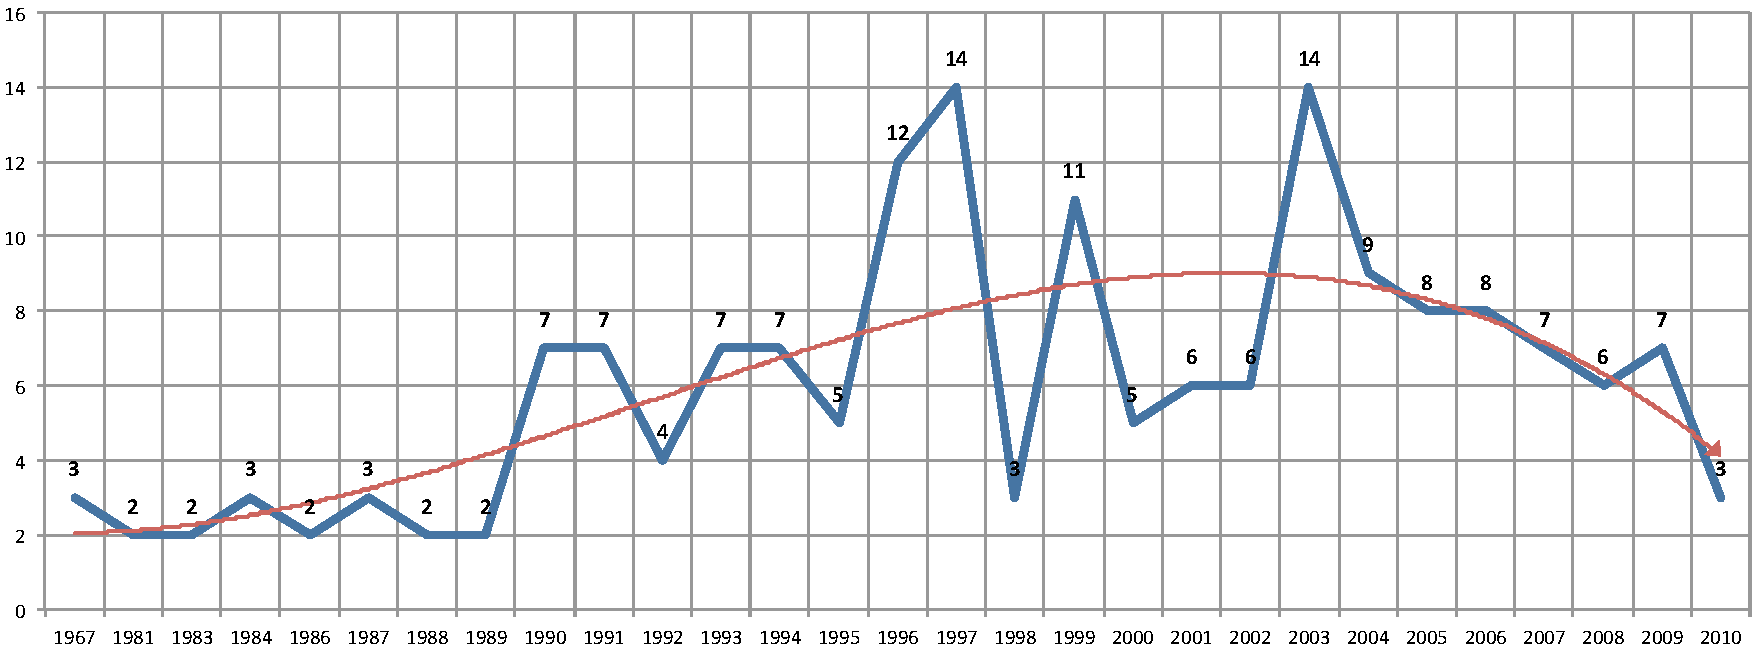
\includegraphics[scale=0.5]{abntex2-modelo-img-grafico.pdf}
	\end{center}
	\legend{Fonte: \citeonline[p. 24]{araujo2012}}
\end{figure}

% ---
\subsection{Figuras em \emph{minipages}}
% ---

\emph{Minipages} são usadas para inserir textos ou outros elementos em quadros
com tamanhos e posições controladas. Veja o exemplo da
\autoref{fig_minipage_imagem1} e da \autoref{fig_minipage_grafico2}.
\begin{figure}[htb]
 \label{teste}
 \centering
  \begin{minipage}{0.45\textwidth}
    \centering
    \caption{Imagem 1 da minipage} \label{fig_minipage_imagem1}
    
\includegraphics[scale=0.8]{abntex2-modelo-img-marca.pdf}
    \legend{Fonte: Produzido pelos autores}
  \end{minipage}
  \hfill
  \begin{minipage}{0.45\textwidth}
    \centering
    \caption{Grafico 2 da minipage} \label{fig_minipage_grafico2}
    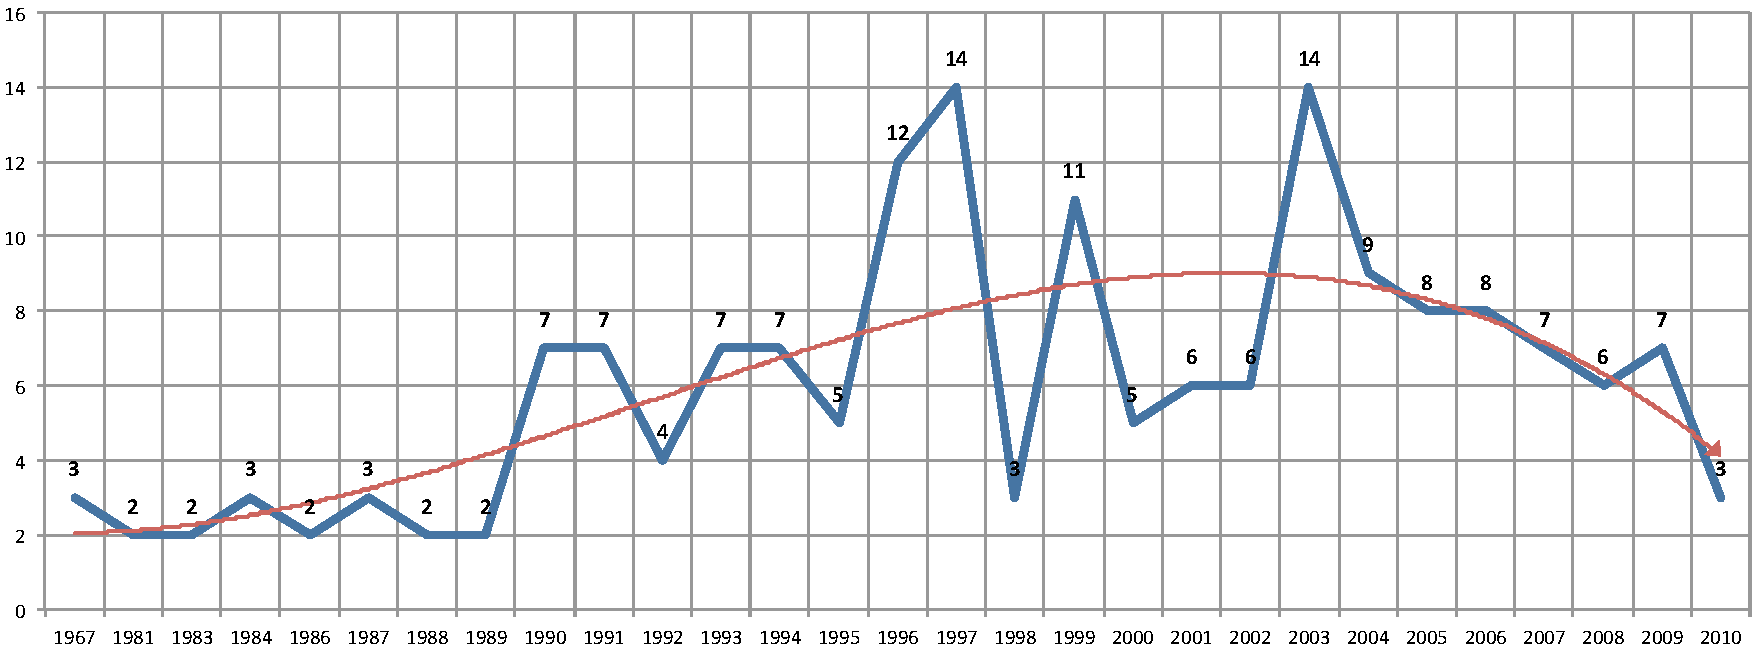
\includegraphics[scale=0.2]{abntex2-modelo-img-grafico.pdf}
    \legend{Fonte: \citeonline[p. 24]{araujo2012}}
  \end{minipage}
\end{figure}

Observe que, segundo a \citeonline[seções 4.2.1.10 e 5.8]{NBR14724:2011}, as
ilustrações devem sempre ter numeração contínua e única em todo o documento:
\begin{citacao}
Qualquer que seja o tipo de ilustração, sua identificação aparece na parte
superior, precedida da palavra designativa (desenho, esquema, fluxograma,
fotografia, gráfico, mapa, organograma, planta, quadro, retrato, figura,
imagem, entre outros), seguida de seu número de ordem de ocorrência no texto,
em algarismos arábicos, travessão e do respectivo título. Após a ilustração, na
parte inferior, indicar a fonte consultada (elemento obrigatório, mesmo que
seja produção do próprio autor), legenda, notas e outras informações
necessárias à sua compreensão (se houver). A ilustração deve ser citada no
texto e inserida o mais próximo possível do trecho a que se
refere. \cite[seção 5.8]{NBR14724:2011}
\end{citacao}

% ---
\section{Subfiguras}
% ---

Como pode ser visto em \citeonline[seção 5.8]{NBR14724:2011}, as subfiguras não 
são elementos regulamentados pelas normas ABNT. A classe \textsf{memoir} dispõe
de comandos para inserção e manejo de subfiguras sem a necessidade de adição de
novos pacotes. Como exemplo, podemos dispor de subfiguras tais como as que seguem
na \autoref{fig_subfigs}, respectivamente as subfiguras \ref{subfig_one} e 
\ref{subfig_two}, juntamente com a \autoref{subfig_three}.
\begin{figure}
  \centering
  \caption{Usando subfiguras}
  \label{fig_subfigs}
  \subtop[\label{subfig_one}Primeira subfigura]{%
    \includegraphics[width=0.3\linewidth]{example-image-a}}
  \subtop[\label{subfig_two}Segunda subfigura]{%
    \includegraphics[width=0.3\linewidth]{example-image-b}}
  \subtop[queisso][\label{subfig_three}Terceira subfigura, com título em mais de uma linha]{%
    \includegraphics[width=0.3\linewidth]{example-image-c}}
  \legend{Fonte: Extraído de \TeX--\LaTeX\ Stack Exchange}
\end{figure}

% ---
\section{Expressões matemáticas}
\label{math-expr}
% ---

\index{expressões matemáticas}Use o ambiente \texttt{equation} para escrever
expressões matemáticas numeradas:
\begin{equation}
  \forall x \in X, \quad \exists \: y \leq \epsilon
\end{equation}

Escreva expressões matemáticas entre \$ e \$, como em $ \lim_{x \to \infty}
\exp(-x) = 0 $, para que fiquem na mesma linha.

Também é possível usar colchetes para indicar o início de uma expressão
matemática que não é numerada.
\[
\left|\sum_{i=1}^n a_ib_i\right|
\le
\left(\sum_{i=1}^n a_i^2\right)^{1/2}
\left(\sum_{i=1}^n b_i^2\right)^{1/2}
\]

Consulte mais informações sobre expressões matemáticas em
\url{https://github.com/abntex/abntex2/wiki/Referencias}.

%---
\section{Teoremas, lemas, proposições e outros ambientes}
% ---

A comunidade matemática utiliza com bastante frequência os ambientes 
\textsf{teorema}, \textsf{lema}, \textsf{proposição} e outros ambientes 
relacionados. Tais definições não necessitam de pacotes adicionais e
podem ser realizadas nas configurações globais.

\begin{definition}[Limite]
  \label{definicao}
  Sejam $f\colon A\rightarrow\mathds{R}$ uma função e $b\in\mathds{R}$ tais 
  que para todo intervalo aberto $I$, contendo $b$, tem-se 
  $I\cap(A-\{b\})\neq\emptyset$. O número real $L$ é o limite de $f(x)$ quando
  $x$ aproxima-se de $b$ quando para todo número $\epsilon>0$, existe $\delta>0$
  ($\delta$ dependendo de $\epsilon$), tal que, se $x\in A$ e $0<|x-b|<\delta$
  então $|f(x)-L|<\epsilon$.
\end{definition}

\begin{proposition}[Unicidade do limnite]
  \label{proposicao}
  Se $\lim_{x\rightarrow b}f(x)=L_1$ e $\lim_{x\rightarrow b}f(x)=L_2$
  ($L_1,L_2\in\mathds{R}$), então $L_1=L_2$.
\end{proposition}

\begin{corollary}
  \label{corolario}
  Se as funções $f(x)$ e $g(x)$ são tais que $f(x) = g(x)$ exceto num ponto $b$,
  então $\lim_{x\rightarrow b}f(x)=\lim_{x\rightarrow b}g(x)$, desde que exista
  um dos limites.
\end{corollary}

\begin{lemma}
  \label{lema}
  Se $a|b$ então $\mathrm{mdc}(a,b)=a$.
\end{lemma}

\begin{theorem}[do Ponto Fixo de Brouwer]
  \label{teorema}
  Se $f\colon[0,1]\rightarrow[0,1]$ é contínua, então $f$ tem ponto fixo.
\end{theorem}
\begin{proof}
  Este ambiente só está definido para o pacote \textsf{amsthm}.
\end{proof}


\begin{conjecture}[de Poincaré]
  \label{conjectura}
  Toda variedade fechada simplesmente conexa de dimensão 3 é equivalente à esfera
  3-dimensional.
\end{conjecture}

% \begin{notation}
%   \label{notacao}
%   oioioi
% \end{notation}

\begin{remark}
  \label{observacao}
  Os gráficos de $f(x) + c$, $f(x + c)$, $cf(x)$ e $f(c x)$ ($c\in\mathds{R}$) 
  podem ser obtidos diretamente do gráfico de $f(x)$.
\end{remark}

% \begin{note}
%   \label{nota}
%   oioioi
% \end{note}

\begin{example}
  \label{exemplo}
  A composta de funções afins é uma função afim.\newline De fato, sejam $f(x)=m_1x+b_1$ e
  $g(x)=m_2x+b_2$. Então, $(g\circ f)(x)=(m_1m_2)x+m_2b_1+b_2$ e 
  $(f\circ g)(x)=(m_1m_2)x+m_1b_2+b_1$.
\end{example}

Para citar no texto, basta usar \textsf{label} dentro de cada ambiente desejado:
\autoref{definicao}, \autoref{proposicao}, \autoref{corolario}, \autoref{lema},
\autoref{teorema}, \autoref{conjectura}, \autoref{observacao}, \autoref{exemplo}.
%, \autoref{}, \autoref{}.

% ---
\section{Enumerações: alíneas e subalíneas}
% ---

\index{alíneas}\index{subalíneas}\index{incisos}Quando for necessário enumerar
os diversos assuntos de uma seção que não possua título, esta deve ser
subdividida em alíneas \cite[4.2]{NBR6024:2012}:
\begin{alineas}
  \item os diversos assuntos que não possuam título próprio, dentro de uma mesma
  seção, devem ser subdivididos em alíneas; 
  
  \item o texto que antecede as alíneas termina em dois pontos;
  \item as alíneas devem ser indicadas alfabeticamente, em letra minúscula,
  seguida de parêntese. Utilizam-se letras dobradas, quando esgotadas as
  letras do alfabeto;

  \item as letras indicativas das alíneas devem apresentar recuo em relação à
  margem esquerda;

  \item o texto da alínea deve começar por letra minúscula e terminar em
  ponto-e-vírgula, exceto a última alínea que termina em ponto final;

  \item o texto da alínea deve terminar em dois pontos, se houver subalínea;

  \item a segunda e as seguintes linhas do texto da alínea começa sob a
  primeira letra do texto da própria alínea;
  
  \item subalíneas \cite[4.3]{NBR6024:2012} devem ser conforme as alíneas a
  seguir:

  \begin{alineas}
     \item as subalíneas devem começar por travessão seguido de espaço;

     \item as subalíneas devem apresentar recuo em relação à alínea;

     \item o texto da subalínea deve começar por letra minúscula e terminar em
     ponto-e-vírgula. A última subalínea deve terminar em ponto final, se não
     houver alínea subsequente;

     \item a segunda e as seguintes linhas do texto da subalínea começam sob a
     primeira letra do texto da própria subalínea.
  \end{alineas}
  
  \item no \abnTeX\ estão disponíveis os ambientes \texttt{incisos} e
  \texttt{subalineas}, que em suma são o mesmo que se criar outro nível de
  \texttt{alineas}, como nos exemplos à seguir:
  
  \begin{incisos}
    \item \textit{Um novo inciso em itálico};
  \end{incisos}
  
  \item Alínea em \textbf{negrito}:
  
  \begin{subalineas}
    \item \textit{Uma subalínea em itálico};
    \item \underline{\textit{Uma subalínea em itálico e sublinhado}}; 
  \end{subalineas}
  
  \item Última alínea com \emph{ênfase}.
  
\end{alineas}

% ---
\section{Espaçamento entre parágrafos e linhas}
% ---

\index{espaçamento!dos parágrafos}O tamanho do parágrafo, espaço entre a margem
e o início da frase do parágrafo, é definido por:
\begin{verbatim}
   \setlength{\parindent}{2.0cm}
\end{verbatim}

\index{espaçamento!do primeiro parágrafo}Por padrão, não há espaçamento no
primeiro parágrafo de cada início de divisão do documento
(\autoref{sec-divisoes}). Porém, você pode definir que o primeiro parágrafo
também seja indentado, como é o caso deste documento. Para isso, apenas inclua o
pacote \textsf{indentfirst} no preâmbulo do documento:
\begin{verbatim}
 \usepackage{indentfirst}    % Indenta o primeiro parágrafo de cada seção.
\end{verbatim}

\index{espaçamento!entre os parágrafos}O espaçamento entre um parágrafo e outro
pode ser controlado por meio do comando:
\begin{verbatim}
  \setlength{\parskip}{0.2cm}  % tente também \onelineskip
\end{verbatim}

\index{espaçamento!entre as linhas}O controle do espaçamento entre linhas é
definido por:
\begin{verbatim}
  \OnehalfSpacing       % espaçamento um e meio (padrão); 
  \DoubleSpacing        % espaçamento duplo
  \SingleSpacing        % espaçamento simples	
\end{verbatim}

Para isso, também estão disponíveis os ambientes:
\begin{verbatim}
  \begin{SingleSpace} ...\end{SingleSpace}
  \begin{Spacing}{hfactori} ... \end{Spacing}
  \begin{OnehalfSpace} ... \end{OnehalfSpace}
  \begin{OnehalfSpace*} ... \end{OnehalfSpace*}
  \begin{DoubleSpace} ... \end{DoubleSpace}
  \begin{DoubleSpace*} ... \end{DoubleSpace*} 
\end{verbatim}

Para mais informações, consulte \citeonline[p. 47-52 e 135]{memoir}.

% ---
\section{Inclusão de outros arquivos}\label{sec-include}
% ---

É uma boa prática dividir o seu documento em diversos arquivos, e não
apenas escrever tudo em um único. Esse recurso foi utilizado neste
documento. Para incluir diferentes arquivos em um arquivo principal,
de modo que cada arquivo incluído fique em uma página diferente, utilize o
comando:
\begin{verbatim}
   \include{documento-a-ser-incluido}      % sem a extensão .tex
\end{verbatim}

Para incluir documentos sem quebra de páginas, utilize:
\begin{verbatim}
   \input{documento-a-ser-incluido}      % sem a extensão .tex
\end{verbatim}

% ---
\section{Compilar o documento \LaTeX}
% ---

Geralmente os editores \LaTeX, como o
TeXlipse\footnote{\url{http://texlipse.sourceforge.net/}}, o
Texmaker\footnote{\url{http://www.xm1math.net/texmaker/}}, entre outros,
compilam os documentos automaticamente, de modo que você não precisa se
preocupar com isso.

No entanto, você pode compilar os documentos \LaTeX usando os seguintes
comandos, que devem ser digitados no \emph{Prompt de Comandos} do Windows ou no
\emph{Terminal} do Mac ou do Linux:
\begin{verbatim}
  pdflatex ARQUIVO_PRINCIPAL.tex
  bibtex ARQUIVO_PRINCIPAL.aux
  makeindex ARQUIVO_PRINCIPAL.idx 
  makeindex ARQUIVO_PRINCIPAL.nlo -s nomencl.ist -o ARQUIVO_PRINCIPAL.nls
  pdflatex ARQUIVO_PRINCIPAL.tex
  pdflatex ARQUIVO_PRINCIPAL.tex
\end{verbatim}

% ---
\section{Remissões internas}
% ---

Ao nomear a \autoref{tab-nivinv} e a \autoref{fig_circulo}, apresentamos
um exemplo de remissão interna que também pode ser feita quando indicamos
o \autoref{cap_exemplos}, que tem o nome \emph{\nameref{cap_exemplos}}.
O número do capítulo indicado é \ref{cap_exemplos}, que se inicia à
\autopageref{cap_exemplos}\footnote{O número da página de uma remissão
pode ser obtida também assim:
\pageref{cap_exemplos}.}.
Veja a \autoref{sec-divisoes} para outros exemplos de remissões internas
entre seções, subseções e subsubseções.

O código usado para produzir o texto desta seção é:
\begin{verbatim}
Ao nomear a \autoref{tab-nivinv} e a \autoref{fig_circulo}, apresentamos
um exemplo de remissão interna que também pode ser feita quando indicamos
o \autoref{cap_exemplos}, que tem o nome \emph{\nameref{cap_exemplos}}.
O número do capítulo indicado é \ref{cap_exemplos}, que se inicia à
\autopageref{cap_exemplos}\footnote{O número da página de uma remissão
pode ser obtida também assim:
\pageref{cap_exemplos}.}.
Veja a \autoref{sec-divisoes} para outros exemplos de remissões internas
entre seções, subseções e subsubseções.
\end{verbatim}

% ---
\section{Divisões do documento: seção}\label{sec-divisoes}
% ---

Esta seção testa o uso de divisões de documentos. Esta é a
\autoref{sec-divisoes}. Veja a \autoref{sec-divisoes-subsection}.

\subsection{Divisões do documento: subseção}\label{sec-divisoes-subsection}

Isto é uma subseção. Veja a \autoref{sec-divisoes-subsubsection}, que é uma
\texttt{subsubsection} do \LaTeX, mas é impressa chamada de ``subseção'' porque
no Português não temos a palavra ``subsubseção''.

\subsubsection{Divisões do documento: subsubseção}
\label{sec-divisoes-subsubsection}

Isto é uma subsubseção.

\subsubsection{Divisões do documento: subsubseção}

Isto é outra subsubseção.

\subsection{Divisões do documento: subseção}\label{sec-exemplo-subsec}

Isto é uma subseção.

\subsubsection{Divisões do documento: subsubseção}

Isto é mais uma subsubseção da \autoref{sec-exemplo-subsec}.


\subsubsubsection{Esta é uma subseção de quinto
nível}\label{sec-exemplo-subsubsubsection}

Esta é uma seção de quinto nível. Ela é produzida com o seguinte comando:
\begin{verbatim}
\subsubsubsection{Esta é uma subseção de quinto
nível}\label{sec-exemplo-subsubsubsection}
\end{verbatim}

\subsubsubsection{Esta é outra subseção de quinto nível}\label{sec-exemplo-subsubsubsection-outro}

Esta é outra seção de quinto nível.


\paragraph{Este é um parágrafo numerado}\label{sec-exemplo-paragrafo}

Este é um exemplo de parágrafo nomeado. Ele é produzida com o comando de
parágrafo:
\begin{verbatim}
\paragraph{Este é um parágrafo nomeado}\label{sec-exemplo-paragrafo}
\end{verbatim}

A numeração entre parágrafos numeradaos e subsubsubseções são contínuas.

\paragraph{Esta é outro parágrafo numerado}\label{sec-exemplo-paragrafo-outro}

Esta é outro parágrafo nomeado.

% ---
\section{Este é um exemplo de nome de seção longo. Ele deve estar
alinhado à esquerda e a segunda e demais linhas devem iniciar logo abaixo da
primeira palavra da primeira linha}
% ---

Isso atende à norma \citeonline[seções de 5.2.2 a 5.2.4]{NBR14724:2011} 
 e \citeonline[seções de 3.1 a 3.8]{NBR6024:2012}.

% ---
\section{Diferentes idiomas e hifenizações}
\label{sec-hifenizacao}
% ---

Para usar hifenizações de diferentes idiomas, inclua nas opções do documento o
nome dos idiomas que o seu texto contém. Por exemplo (para melhor
visualização, as opções foram quebras em diferentes linhas):
\begin{verbatim}
\documentclass[
	12pt,
	openright,
	twoside,
	a4paper,
	english,
	spanish,
	brazil
	]{abntex2}
\end{verbatim}

O idioma português-brasileiro (\texttt{brazil}) é incluído automaticamente pela
classe \textsf{abntex2}. Porém, mesmo assim a opção \texttt{brazil} deve ser
informada como a última opção da classe para que todos os pacotes reconheçam o
idioma. Vale ressaltar que a última opção de idioma é a utilizada por padrão no
documento. Desse modo, caso deseje escrever um texto em inglês que tenha
citações em português e em espanhol, você deveria usar o preâmbulo como abaixo:
\begin{verbatim}
\documentclass[
	12pt,
	openright,
	twoside,
	a4paper,
	spanish,
	brazil,
	english
	]{abntex2}
\end{verbatim}

A lista completa de idiomas suportados, bem como outras opções de hifenização,
estão disponíveis em \citeonline[p.~5-6]{babel}.

Exemplo de hifenização em inglês\footnote{Extraído de:
\url{http://en.wikibooks.org/wiki/LaTeX/Internationalization}}:

\begin{otherlanguage*}{english}
\textit{Text in English language. This environment switches all language-related
definitions, like the language specific names for figures, tables etc. to the other
language. The starred version of this environment typesets the main text
according to the rules of the other language, but keeps the language specific
string for ancillary things like figures, in the main language of the document.
The environment hyphenrules switches only the hyphenation patterns used; it can
also be used to disallow hyphenation by using the language name
`nohyphenation'.}
\end{otherlanguage*}

% Pequeno texto em espanhol\footnote{Extraído de:
% \url{http://internacional.elpais.com/internacional/2013/02/17/actualidad/1361102009_913423.html}}:
% 
% \foreignlanguage{spanish}{\textit{Decenas de miles de personas ovacionan al pontífice en su
% penúltimo ángelus dominical, el primero desde que anunciase su renuncia. El Papa se
% centra en la crítica al materialismo}}.

O idioma geral do texto por ser alterado como no exemplo seguinte:
\begin{verbatim}
  \selectlanguage{english}
\end{verbatim}

Isso altera automaticamente a hifenização e todos os nomes constantes de
referências do documento para o idioma inglês. Consulte o manual da classe
\cite{abntex2classe} para obter orientações adicionais sobre internacionalização de
documentos produzidos com \abnTeX.

A \autoref{sec-citacao} descreve o ambiente \texttt{citacao} que pode receber
como parâmetro um idioma a ser usado na citação.

% ---
\section{Consulte o manual da classe \textsf{abntex2}}
% ---

Consulte o manual da classe \textsf{abntex2} \cite{abntex2classe} para uma
referência completa das macros e ambientes disponíveis. 

Além disso, o manual possui informações adicionais sobre as normas ABNT
observadas pelo \abnTeX\ e considerações sobre eventuais requisitos específicos
não atendidos, como o caso da \citeonline[seção 5.2.2]{NBR14724:2011}, que
especifica o espaçamento entre os capítulos e o início do texto, regra
propositalmente não atendida pelo presente modelo.

% ---
\section{Referências bibliográficas}
% ---

A formatação das referências bibliográficas conforme as regras da ABNT são um
dos principais objetivos do \abnTeX. Consulte os manuais
\citeonline{abntex2cite} e \citeonline{abntex2cite-alf} para obter informações
sobre como utilizar as referências bibliográficas.

ATENÇÃO: a utilização do comando \textsf{citeonline} em vez de \textsf{cite} só
é permitida quando utiliza-se o pacote \textsf{abntex2cite}!

%-
\subsection{Acentuação de referências bibliográficas}
%-

Normalmente não há problemas em usar caracteres acentuados em arquivos
bibliográficos (\texttt{*.bib}). Porém, como as regras da ABNT fazem uso quase
abusivo da conversão para letras maiúsculas, é preciso observar o modo como se
escreve os nomes dos autores. Na ~\autoref{tabela-acentos} você encontra alguns
exemplos das conversões mais importantes. Preste atenção especial para `ç' e `í'
que devem estar envoltos em chaves. A regra geral é sempre usar a acentuação
neste modo quando houver conversão para letras maiúsculas.
\begin{table}[htbp]
\caption{Tabela de conversão de acentuação.}
\label{tabela-acentos}
\begin{center}
\begin{tabular}{ll}\hline\hline
acento & \textsf{bibtex}\\
à á ã & \verb+\`a+ \verb+\'a+ \verb+\~a+\\
í & \verb+{\'\i}+\\
ç & \verb+{\c c}+\\
\hline\hline
\end{tabular}
\end{center}
\end{table}

% ---
\section{Referências cruzadas (cross referencing)}
% ---

A classe \abnTeX\ permite o uso do comando \textsf{autoref} para referenciar 
diversos itens do texto produzido, como capítulos e seções, figuras, tabelas, 
equações, algoritmos e códigos. A partir de um \textsf{label} fornecido, basta 
utilizar o comando para referenciar algo do texto.

Como exemplo, podemos citar a \autoref{tabela-acentos}, a 
\autoref{fig_grafico}, a \autoref{math-expr} e o \autoref{chpt2}.
Sem o \textsf{autoref} a saída se torna a Tabela 
\ref{tabela-acentos}, a Figura \ref{fig_grafico}, a seção 
\ref{math-expr} e o Capítulo \ref{chpt2}.

O código que gerou o parágrafo anterior foi:
\begin{verbatim}
Como exemplo, podemos citar a \autoref{tabela-acentos}, a 
\autoref{fig_grafico}, a \autoref{math-expr} e o \autoref{chpt2}.
Sem o \textsf{autoref} a saída se torna a Tabela 
\ref{tabela-acentos}, a Figura \ref{fig_grafico}, a seção 
\ref{math-expr} e o Capítulo \ref{chpt2}.
\end{verbatim}

Perceba a necessidade de inserir o label a que se refere a referência
(Tabela, Figura, Capítulo) quando não usamos o comando \textsf{autoref}.

% ----------------------------------------------------------
% ----------------------------------------------------------

\chapter{Exemplo de um texto de título que pode ser bastante longo e sua sugestão
de solução para evitar problemas com o cabeçalho}
\label{chpt2}

Note, na página seguinte, que há um problema na disposição textual dos
itens do cabeçalho. O cabeçalho está ocupando mais de uma linha e a numeração
de página está ficando ao final do cabeçalho, com alinhamento à direita.

Ocorre que, para a secretaria da pós-graduação do IMECC, isso é um problema e
o texto não será aceito. Uma sugestão é usar títulos mais curtos para utilização
nos cabeçalhos.

Observe que o comando \verb|\chapter[*]{*}| possui dois argumentos: o primeiro
argumento é uma versão mais curta do texto do título e o segundo argumento é uma
versão mais completa do texto do título do capítulo:
\begin{verbatim}
    \chapter[<título curto>]{<título completo>}
\end{verbatim}
Com esse formato, você pode notar que o \verb|<título completo>| é aquele impresso
na página de corpo de texto, enquanto que o \verb|<título curto>| é usado tanto no
sumário quanto nos cabeçalhos. Há uma outra opção que você pode utilizar:
\begin{verbatim}
\chapter[<título sumário>]{<título completo>}  
\chaptermark{<título cabeçalho>}
\end{verbatim}
Desta forma, você consegue definir o texto do título do capítulo que deve ser impresso
em cada parte: sumário, corpo do texto e cabeçalho. Fonte: \url{http://www.texfaq.org/FAQ-runheadtoobig}.

Essa sugestão de correção está implementada para o próximo capítulo.

\lipsum[28-35]

% ----------------------------------------------------------
% ----------------------------------------------------------

\chapter[Exemplo de um título longo e a solução com o cabeçalho]{Exemplo de um texto
de título que pode ser bastante longo e sua sugestão de solução para evitar problemas
com o cabeçalho}
\chaptermark{Cabeçalho com título mais curto}

Observe esta solução a partir do texto que se apresenta para o capítulo no sumário,
no cabeçalho e no corpo do texto.

\lipsum[42-51]

% ----------------------------------------------------------
% ----------------------------------------------------------
% ----------------------------------------------------------
% ----------------------------------------------------------

\part{Referenciais teóricos}

\lipsum[55-64]

% ----------------------------------------------------------
% ----------------------------------------------------------

\part{Resultados}

% ----------------------------------------------------------
% ----------------------------------------------------------
% ----------------------------------------------------------

% ---
\chapter{Algoritmos e códigos-fonte}
% ---

\section{O pacote algorithm2e}

O \textsf{algorithm2e} é um ambiente para escrever algoritmos. Um algoritmo se 
torna um objeto flutuante (como uma figura, tabela, etc.).

\begin{algorithm}
\caption{Primeiro exemplo de algoritmo com uma legenda contendo um texto muito longo que pode ocupar mais de uma linha.\label{IR}}
\KwData{$G=(X,U)$ such that $G^{tc}$ is an order.}
\KwResult{$G'=(X,V)$ with $V\subseteq U$ such that $G'^{tc}$ is an interval order.}
\Begin{
    $V \longleftarrow U$\;
    $S \longleftarrow \emptyset$\;
    \For{$x\in X$}{
	$NbSuccInS(x) \longleftarrow 0$\;
	$NbPredInMin(x) \longleftarrow 0$\;
	$NbPredNotInMin(x) \longleftarrow |ImPred(x)|$\;
    }
    \For{$x \in X$}{
	\If{$NbPredInMin(x) = 0$ \textnormal{\textbf{and}} $NbPredNotInMin(x) = 0$}{$AppendToMin(x)$}
    }
    \nl\While{$S \neq \emptyset$}{\label{InRes1}
	\nlset{REM} remove $x$ from the list of $T$ of maximal index\;\label{InResR}
	\lnl{InRes2}\While{$|S \cap  ImSucc(x)| \neq |S|$}{
	    \For{$ y \in  S-ImSucc(x)$}{
		\{ remove from $V$ all the arcs $zy$ : \}\;
		\For{$z \in  ImPred(y) \cap  Min$}{
		    remove the arc $zy$ from $V$\;
		    $NbSuccInS(z) \longleftarrow NbSuccInS(z) - 1$\;
		    move $z$ in $T$ to the list preceding its present list\;
		    \{i.e. If $z \in T[k]$, move $z$ from $T[k]$ to
		    $T[k-1]$\}\;
		}
		$NbPredInMin(y) \longleftarrow 0$\;
		$NbPredNotInMin(y) \longleftarrow 0$\;
		$S \longleftarrow S - \{y\}$\;
		$AppendToMin(y)$\;
	    }
	}
	$RemoveFromMin(x)$\;
    }
}
\end{algorithm}

Como pode ser visto na documentação do pacote \textsf{algorithm2e} (informações
em  \url{https://www.ctan.org/pkg/algorithm2e}), o pacote não oferece comandos 
para quebra de página, caso seu algoritmo ocupe mais de uma página. Em muitos
casos, este inconveniente pode ser facilmente contornado alterando o tamanho a
fonte utilizada no ambiente. O ponto forte deste pacote é que ele é um pacote 
que  possui atualizações periódicas, sendo a última versão a 5.1 datada de 10 
de novembro de 2015 (Manter todo o sistema \LaTeX\ atualizado é vital para o 
bom funcionamento de todos os pacotes e comandos utilizados: mantenha seu 
sistema sempre atualizado!).

\setcounter{algocf}{98}

\begin{algorithm}
\SetAlgoLined
\KwData{this text}
\KwResult{how to write algorithm with \LaTeX2e }
initialization\;
\While{not at end of this document}{
read current\;
\eIf{understand}{
go to next section\;
current section becomes this one\;
}{
go back to the beginning of current section\;
}
}
\caption{How to write algorithms.}
\end{algorithm}

\section{O pacote listings}

O pacote permite que o usuário escreva programas (código de programação) dentro
do \LaTeX; O código-fonte é lido diretamente pelo TeX-nenhum processador front-end
é necessário. Palavras-chave, comentários e seqüências de caracteres podem ser 
composta usando estilos diferentes (padrão é negrito para palavras-chave, itálico
para comentários e nenhum estilo especial para seqüências de caracteres). Suporte
para hyperref é fornecido (informações em \url{https://www.ctan.org/pkg/listings}).

\begin{lstlisting}[caption={Exemplo de código em C++ usando o pacote \texttt{listings} e que tem título longo ocupando mais de uma linha},label=ex-listing]
#include 
using namespace std;
int main()
{
  /* comentario */
  int n, i, a = 0, b = 1, F;
  cout << "Digite o numero de termos da sequencia de Fibonacci: ";
   cin >> n;
  cout << a << " " << b << " ";
   for (i = 0; i < n - 2; i++)   {
     F = a + b;
     cout << F << " ";
     a = b;
     b = F;
   } cout << endl; return 0;
 }
\end{lstlisting}

Diferentemente do pacote \textsf{algorithm2e}, o pacote \textsf{listings} não
possui problemas com quebra de páginas para códigos computacionais que ocupem
mais de uma página.

\setcounter{lstlisting}{98}

\begin{lstlisting}[caption=Exemplo de código em C++ usando o pacote \texttt{listings},label=ex-listing-two]
#include 
using namespace std;
int main()
{
  /* comentario */
  int n, i, a = 0, b = 1, F;
  cout << "Digite o numero de termos da sequencia de Fibonacci: ";
   cin >> n;
  cout << a << " " << b << " ";
   for (i = 0; i < n - 2; i++)   {
     F = a + b;
     cout << F << " ";
     a = b;
     b = F;
   } cout << endl; return 0;
 }
\end{lstlisting}
% ---
% --------------------
% FIM DOS EXEMPLOS
% --------------------
% ----------------------------------------------------------
% CONSIDERAÇÕES FINAIS
% Finaliza a parte no bookmark do PDF para que se inicie o
% bookmark na raiz e adiciona espaço de parte no Sumário
% \phantompart
\chapter{Considerações Finais}

Precisa de ajuda?

Consulte os manuais \abnTeX\ \cite{abntex2classe,abntex2cite,abntex2cite-alf} e da classe \textsf{memoir} \cite{memoir}.

Envie um e-mail para \texttt{gfabinhomat@gmail.com} (Fábio Rodrigues Silva), que é o responsável pela manutenção desta versão de adaptação do modelo canônico \abnTeX.

Consulte a FAQ com perguntas frequentes e comuns no portal do \abnTeX:
\url{https://github.com/abntex/abntex2/wiki/FAQ}.

Inscreva-se no grupo de usuários \LaTeX: \url{http://groups.google.com/group/latex-br}, tire suas dúvidas e ajude outros usuários.

Participe também do grupo de desenvolvedores do \abnTeX: \url{http://groups.google.com/group/abntex2} e faça sua contribuição à ferramenta.
% ----------------------------------------------------------
% ---------------------------------------------------------------------------------
% %%%%%%%%%%%%%%%%%%%%%%%%%% FIM DOS ELEMENTOS TEXTUAIS %%%%%%%%%%%%%%%%%%%%%%%%%%
% ---------------------------------------------------------------------------------
% ---------------------------------------------------------------------------------
% %%%%%%%%%%%%%%%%%%%%%%% INÍCIO DOS ELEMENTOS PÓS-TEXTUAIS %%%%%%%%%%%%%%%%%%%%%%%
% ---------------------------------------------------------------------------------
% ----------------------------------------------------------
\postextual
% ----------------------------------------------------------
% ----------------------------------------------------------
% REFERÊNCIAS
\nocite{masolo2010}
\bibliography{abntex2-modelo-references}
% ----------------------------------------------------------
% ----------------------------------------------------------
% APÊNDICES
\begin{apendicesenv}
% Imprime uma página indicando o início dos apêndices
\partapendices
\chapter{Quisque libero justo}

\lipsum[50]

\chapter{Nullam elementum urna vel imperdiet sodales elit ipsum pharetra ligula
ac pretium ante justo a nulla curabitur tristique arcu eu metus}

\lipsum[55-57]
\end{apendicesenv}
% ----------------------------------------------------------
% ----------------------------------------------------------
% ANEXOS
\begin{anexosenv}
% Imprime uma página indicando o início dos anexos
\partanexos
\chapter{Morbi ultrices rutrum lorem.}

\lipsum[30]

\chapter{Cras non urna sed feugiat cum sociis natoque penatibus et magnis dis
parturient montes nascetur ridiculus mus}

\lipsum[31]

\chapter{Fusce facilisis lacinia dui}

\lipsum[32]
\end{anexosenv}
% ----------------------------------------------------------
% ----------------------------------------------------------
% ---------------------------------------------------------------------------------
% %%%%%%%%%%%%%%%%%%%%%%%%%% FIM DOS ELEMENTOS TEXTUAIS %%%%%%%%%%%%%%%%%%%%%%%%%%
% ----------------------------------------------------------------------------------
% -----------------------------------------------------------------------------------------------
% %%%%%%%%%%%%%%%%%%%%%%%%%%%%%%%%%%%%%% FIM DO DOCUMENTO %%%%%%%%%%%%%%%%%%%%%%%%%%%%%%%%%%%%%%
% -----------------------------------------------------------------------------------------------
\end{document}